\documentclass[journal,twoside,web]{ieeecolor}
% \documentclass[12pt,peerreview,draftversion,onecolumn,print]{ieeecolor}
\usepackage[table,x11names,svgnames,dvipsnames]{xcolor}
\usepackage[export]{adjustbox}
\usepackage{algorithm}
\usepackage[noend]{algpseudocode}
\usepackage{amsmath,amssymb,amsfonts}
\usepackage[USenglish]{babel}
\usepackage{booktabs}
\usepackage{cancel}
\usepackage[tableposition=above]{caption}
% \usepackage{centernot}
% \usepackage{comment}
% \usepackage{enumitem}
\usepackage{epsfig}
\usepackage{epstopdf}
% \usepackage[letterpaper, top=1.0in, bottom=1.0in, left=1.0in, right=1.0in]{geometry}
\RequirePackage[OT1]{fontenc}
% \usepackage{fontspec}
\usepackage{graphics}
\usepackage{graphicx}
\graphicspath{{figures/}}
% \usepackage{ifpdf}
% \usepackage{lastpage}
% \usepackage{leftidx}
\usepackage{lipsum}
% \usepackage{mathrsfs}
\usepackage{mathtools}
% \usepackage{multicol}
% \usepackage{multirow}
\usepackage{nicefrac}
% \usepackage{nicematrix}
% \usepackage{pgfplots}
\usepackage{pifont}
% \usepackage{ragged2e}
% \usepackage{rotating}
% \usepackage{stmaryrd}
\usepackage[caption=false]{subfig}
\usepackage{tabularx}
\usepackage{tikz}
% \usepackage{tkz-euclide}
% \usepackage{ctable}
% \usetikzlibrary{matrix, arrows}
\usetikzlibrary{shapes.geometric, arrows}
\usepackage{todonotes}
% \usepackage{wrapfig}

\tikzstyle{startstop} = [rectangle, rounded corners, minimum width=1cm, minimum
height = 0.5cm, text centered, draw=black, fill=red!30]
\tikzstyle{io} = [trapezium, trapezium left angle=70, trapezium right angle=110,
minimum height=1cm, text width=3cm, text centered, draw=black, fill=blue!30]
\tikzstyle{process} = [rectangle, minimum width=2cm, minimum height=0.8cm, text
centered, text width=2cm, draw=black, fill=orange!30]
\tikzstyle{decision} = [diamond, aspect=1.25, minimum width=2cm, minimum height=0.5cm, 
text centered, text width=3cm, draw=black, fill=green!30]
\tikzstyle{arrow} = [thick, ->, >=stealth]




\makeatletter
\newcommand{\rmnum}[1]{\romannumeral #1}
\newcommand{\Rmnum}[1]{\expandafter\@slowromancap\romannumeral #1@}
\makeatother

\newcommand{\bmat}[1]{\begin{bmatrix}#1\end{bmatrix}}
\newcommand{\pmat}[1]{\begin{pmatrix}#1\end{pmatrix}}
\newcommand{\ubar}[1]{\text{\b{$#1$}}}
\newcommand{\norm}[2]{\|{#1}\|_{{}_{#2}}}
\newcommand{\abs}[1]{\left|{#1}\right|}
\newcommand{\mbf}[1]{\mathbf{#1}}
\newcommand{\mc}[1]{\mathcal{#1}}
\newcommand{\dd}{\operatorname{d}\!}
\newcommand{\muc}[2]{\multicolumn{#1}{c}{#2}}
\newcommand*\Eval[3]{\left.#1\right\rvert_{#2}^{#3}}
\newcommand{\inner}[1]{\left\langle#1\right\rangle}
\newcommand{\pd}[2]{\frac{\partial #1}{\partial #2}}
\newcommand{\pdd}[2]{\frac{\partial^2 #1}{\partial #2^2}}
\newcommand{\el}[2]{\frac{\dd}{\dd t}\pd{\mc{L}}{\dot{#1}} - \pd{\mc{L}}{#1} = #2}
\newcommand{\elk}[2]{\frac{\dd}{\dd t}\pd{\mc{L}}{\dot{#1}_k} - \pd{\mc{L}}{#1_k} = #2_k}
\newcommand{\vectornorm}[1]{\left|\left|#1\right|\right|}
\newcommand{\dom}[1]{\textrm{dom}\;#1}
\newcommand{\bx}{{\bf x}}
\newcommand{\bu}{{\bf u}}
\newcommand{\cmark}{\ding{51}}%
\newcommand{\xmark}{\ding{55}}%

\newcommand{\idapbc}{\textsc{IdaPbc}}

% \theoremstyle{plain}
% \newtheorem{thm}{Theorem}[section]
% \makeatletter
% \@addtoreset{thm}{section}
% \makeatother
% \newtheorem{cor}[thm]{Corollary}
% \newtheorem{lem}[thm]{Lemma}
% \newtheorem{claim}[thm]{Claim}
% \newtheorem{axiom}[thm]{Axiom}
% \newtheorem{conj}[thm]{Conjecture}
% \newtheorem{fact}[thm]{Fact}
% \newtheorem{hypo}[thm]{Hypothesis}
% \newtheorem{assum}[thm]{Assumption}
\newtheorem{prop}{Proposition}
% \newtheorem{crit}[thm]{Criterion}
% \theoremstyle{definition}
% \newtheorem{defn}[thm]{Definition}
% \newtheorem{exmp}[thm]{Example}
\newtheorem{rem}{Remark}
% \newtheorem{prin}[thm]{Principle}

\DeclareMathOperator{\Tr}{tr}
\newcommand\xdownarrow[1][2ex]{%
   \mathrel{\rotatebox{90}{$\xleftarrow{\rule{#1}{0pt}}$}}
}
\DeclareMathOperator{\End}{End}
\DeclareMathOperator{\Hom}{Hom}
\DeclareMathOperator{\id}{id}
\DeclareMathOperator{\vers}{vers}
\DeclareMathOperator{\trans}{Trans}
\DeclareMathOperator{\rot}{Rot}
\DeclareMathOperator{\rank}{rank}
\DeclareMathOperator{\sinc}{sinc}

%% The section below needs to be put at the end of this file to make citation links work with ieeeconf.cls
\makeatletter
\let\NAT@parse\undefined
\makeatother
\usepackage{hyperref}
\hypersetup{
    unicode=false,          % non-Latin characters in Acrobat’s bookmarks
    pdftoolbar=true,        % show Acrobat’s toolbar?
    pdfmenubar=true,        % show Acrobat’s menu?
    pdffitwindow=false,     % window fit to page when opened
    pdfstartview={FitH},    % fits the width of the page to the window
    pdftitle={Robust Interconnection and Damping Assignment Passivity-Based Control via Neural Bayesian Inference},    % title
    pdfauthor={Wankun Sirichotiyakul, Nardos Ayele Ashenafi, Aykut C. Satici},     % author
    % pdfsubject={Subject},   % subject of the document
    % pdfcreator={Creator},   % creator of the document
    % pdfproducer={Producer}, % producer of the document
    % pdfkeywords={keyword1, key2, key3}, % list of keywords
    pdfnewwindow=true,      % links in new PDF window
    colorlinks=true,       % false: boxed links; true: colored links
    linkcolor=magenta,          % color of internal links (change box color with linkbordercolor)
    linkbordercolor=orange,
    citecolor=blue,        % color of links to bibliography
    citebordercolor=green,
    filecolor=magenta,      % color of file links
    urlcolor=cyan,           % color of external links
    urlbordercolor=blue,
}

\usepackage{generic}

% Not sure if needed
\def\BibTeX{{\rm B\kern-.05em{\sc i\kern-.025em b}\kern-.08em
    T\kern-.1667em\lower.7ex\hbox{E}\kern-.125emX}}

\markboth{\journalname, VOL. XX, NO. XX, February 2023}
{Satici: Estimation of the Parameters of a Second-Order Linear System
(February 2023)}

\begin{document}

\title{Estimation of the Parameters of a Second-Order Linear System} 
\author{
    Aykut C. Satici, \IEEEmembership{Member, IEEE}
    \thanks{Not submitted for review in February 2023.}
    \thanks{A. C. Satici is with the Mechanical and Biomedical Engineering Department, Boise State University, Boise, ID 83706 USA
    (e-mail: aykutsatici@boisestate.edu).}
}
\maketitle
% \IEEEpeerreviewmaketitle

  
\begin{abstract} % Abstract of not more than 200 words.
We study the estimation of the parameters of a second-order linear ODE system
using an adaptation law.
\end{abstract}

\begin{IEEEkeywords}
    Adaptive control, estimation
\end{IEEEkeywords}

\section{Introduction}
\label{sec:intro}

We provide a Lyapunov analysis~\cite{khalil2015nonlinear} to prove that our
control and adaptation laws will stabilize the system to a reference trajectory
while the estimates of the parameters tend to their correct values.

\section{Analysis} 
\label{sec:analysis}

\noindent Consider the scalar linear system with equations of motion given by
the ODE
%
\begin{equation}
    m \ddot{x} + b\dot{x} + kx = u(x, \dot{x}),
    \label{eq:eom}
\end{equation}
%
where $u(x, \dot{x})$ is a control input that is to be determined for tracking.
We are uncertain of the constant parameters $\theta = \bmat{m & b & k}^\top$,
whose estimates are denoted by $\hat{\theta} \in \mathbb{R}^3$. Let us introduce
the errors in the position $x$, and parameters $\theta$ to be \[ \tilde{x} = x -
x_r, \quad \tilde{\theta} = \theta - \hat{\theta}, \] where $x_r$ is a reference
signal for the motion of the mechanical system. Inspired by Chapter 9
of~\cite{spong2020robot}, let us choose the control input according to 
\begin{align}
    \begin{split}
        u(x, \dot{x}) &= Y(x, \dot{x}, a, v)\hat{\theta} - cr, \\
        Y(x, \dot{x}, a, v) &= \bmat{a & v & x},
    \end{split}
    \label{eq:ctrl_law}
\end{align}
%
where the quantities $v$, $a$, and $r$ are given as
\begin{align*}
    v &= \dot{x}_r - \lambda \tilde{x}, \\
    a &= \dot{v} = \ddot{x}_r - \lambda \dot{\tilde{x}}, \\
    r &= \dot{x} - v = \dot{\tilde{x}} + \lambda \tilde{x},
\end{align*}
%
where $c, \lambda > 0$ are constant gains. Substituting the control
law~\eqref{eq:ctrl_law} into the system model~\eqref{eq:eom} leads to
%
\begin{equation}
    m\dot{r} + (b+c)r = -Y\tilde{\theta}.
    \label{eq:control_applied}
\end{equation}
%
The parameter estimate $\hat{\theta}$ may be computed using standard methods of
adaptive control such as gradients or least squares. For example, for a positive
definite matrix $\Gamma$ of appropriate dimensions, we can use the gradient
update law
%
\begin{equation}
    \dot{\hat{\theta}} = -\Gamma^{-1}Y^\top(x, \dot{x}, a, v)r.
    \label{eq:param_update}
\end{equation}

Consider the Lyapunov function candidate
%
\begin{equation*}
    V(\tilde{x}, \dot{\tilde{x}}, \tilde{\theta}) = \frac{1}{2}mr^2 + 
    c\lambda\tilde{x}^2 + \frac{1}{2}\tilde{\theta}^\top\Gamma\tilde{\theta}.
%     \label{eq:lyap_cand}
\end{equation*}
%
This is a positive definite function over the space of $\pmat{\tilde{x},
\dot{\tilde{x}}, \tilde{\theta}}$. We take the time derivative of the Lyapunov
function candidate and substitute from the closed-loop system
dynamics~(\ref{eq:control_applied}, \ref{eq:param_update}). We suppress its
functional dependence for brevity.
%
\begin{align*}
    \dot{V} &= mr\dot{r} + 2c\lambda \tilde{x}\dot{\tilde{x}} +
    \tilde{\theta}^\top\Gamma\dot{\tilde{\theta}} \\
            &= r\left(-(b+c)r - Y\tilde{\theta}\right) + 2c\lambda
            \tilde{x}\dot{\tilde{x}} + \tilde{\theta}^\top Y^\top r \\
            &= -c\lambda^2\tilde{x}^2 - c\dot{\tilde{x}}^2 - br^2 \leq 0.
\end{align*}
%
Hence the set $\Omega_c = \{(\tilde{x}, \dot{\tilde{x}}, \tilde{\theta}):
V(\tilde{x}, \dot{\tilde{x}}, \tilde{\theta}) \leq c \}$ is positively
invariant for any $c > 0$. Moreover, $\tilde{x}, \dot{\tilde{x}}, r \rightarrow
0$ as $t \rightarrow \infty$. This means $u(x, \dot{x}) \rightarrow
\hat{m}\ddot{x}_r + \hat{b}\dot{x}_r + \hat{k}x_r$ (since $x \rightarrow x_r$).
We identify $S = \{(\tilde{x}, \dot{\tilde{x}}, \tilde{\theta}): (\tilde{x},
\dot{\tilde{x}}) = 0\}$ as the set of all points in $\Omega_c$ where $\dot{V} =
0$. We now show that for a specific choice of the reference signal $x_r(t)$, no
solution can stay identically in $S$ other than the trivial solution
$(\tilde{x}, \dot{\tilde{x}}, \tilde{\theta}) = (0,0,0)$ and invoke Corollary
4.1 of~\cite{khalil2015nonlinear} proving that the errors converge to zero.

To this end, for any solution that belongs identically to $S$, the system
dynamics yields \[ \tilde{m}\ddot{x}_r + \tilde{b}\dot{x}_r + \tilde{k}x_r
\equiv 0, \qquad \dot{\tilde{m}} \equiv \dot{\tilde{b}} \equiv \dot{\tilde{k}}
\equiv 0. \] 
%
Excite several frequencies by choosing 
\begin{align*}
    x_r(t) &= A\sin{\left(\omega(t) + \varphi\right)} \\
    \omega(t) &= \sum_{k=1}^n \left(1-\frac{k-1}{n}\right)\sin{k t}
\end{align*}
%
for some constants $A > 0$, $n \in \mathbb{N}$ and $\varphi$. Choosing $n$
sufficiently large, we excite enough frequencies so that $\tilde{\theta}
\rightarrow 0$, making the origin of $(\tilde{x}, \dot{\tilde{x}},
\tilde{\theta})$ globally asymptotically stable.

\section{Results}
\label{sec:results}

\begin{figure}[b]
  \centering
  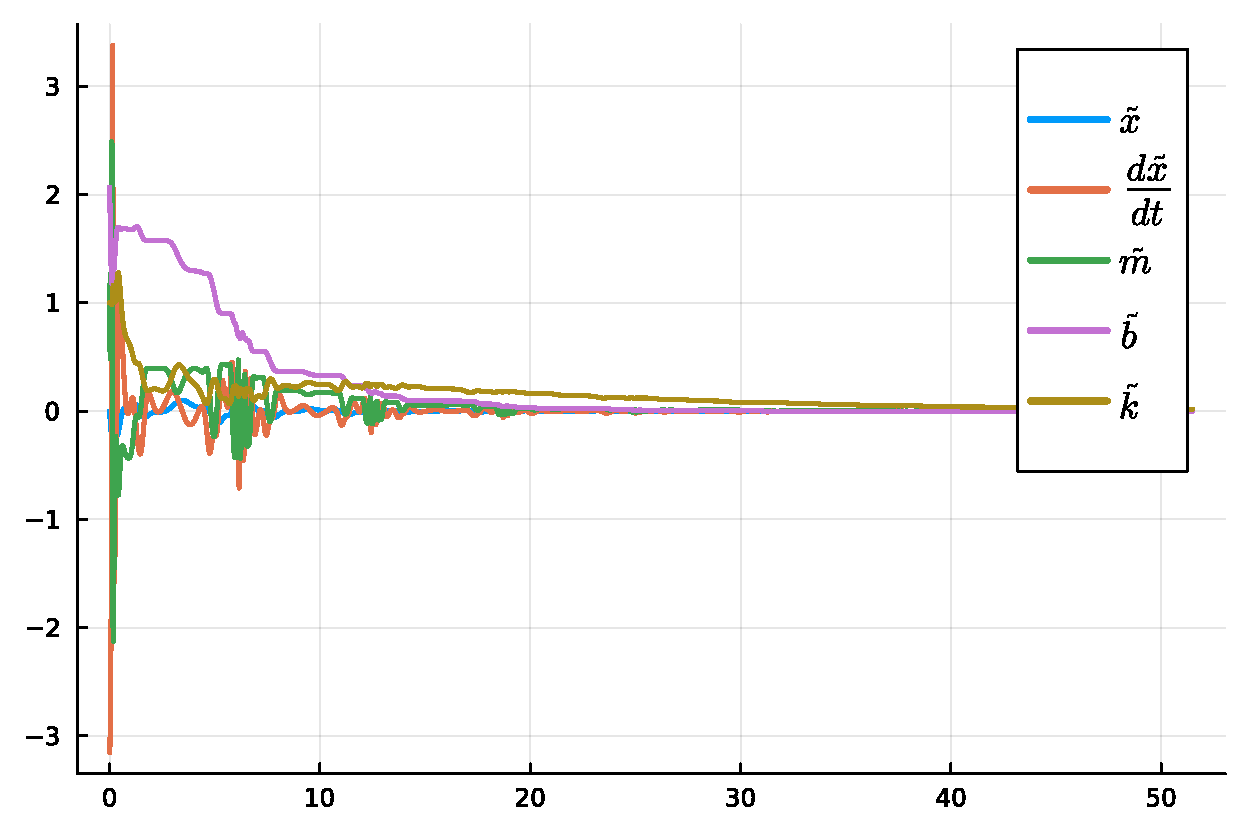
\includegraphics[width=0.5\textwidth]{./figures/adaptationrule2.pdf}
  \caption{Simulation showing the convergence of the system state and parameter
  estimates.}
  \label{fig:adaptation}
\end{figure}

In Figure~\ref{fig:adaptation}, we plot the response of the system to the
control and adaptation laws~(\ref{eq:ctrl_law}, \ref{eq:param_update}),
implemented in simulation. The constants that are used are as follows: $(A, n,
\varphi) = (\nicefrac{3}{10}, 3, 0^\circ)$ and $(c, \lambda) = (1, 4)$. The real
mass, damping and stiffness of the system are $(m, b, k) = (0.665, 1.819, 0)$
and their estimates start at $(\hat{m}, \hat{b}) = (-\nicefrac{1}{2},
-\nicefrac{1}{4}, -1)$.

\section{Conclusion}
\label{sec:conclusion}

We have shown that our control and adaptation laws for the linear second-order
mechanical system guide the estimates of the parameters to tend to their correct
values while tracking a judiciously chosen reference signal.


\bibliographystyle{ieeetr}        
\bibliography{bib/references.bib}  

% \appendix

\newcommand*{\bbU}{\mathbb{U}}

\section{Supplementary Stability Discussions}

\subsection{Proof of Proposition~\ref{prop:control_continuous}}
\label{appendix:proof_control_continuous}

\begin{proof}
    Let $\bbU = \bbU(\theta)$ denote the right side of
    equation~\eqref{eq:Gues}. 
    %
    In this notation, the objective function of~\eqref{eq:finite_optim}
    is the squared norm of $G^{\perp} \bbU$. 
    %
    Let $(\cdot)^{(k)}$ denote the $k^{\textrm{th}}$ iteration of the
    optimization algorithm.
    %
    Since 
    $J^{(k)} \to 0,\, \bbU^{(k)} \to \bbU^{\star}$, 
    and
    $\theta^{(k)} \to \theta^{\star}$, 
    there exists an integer $K>0$ such that when $k > K$, the following are true:
    %
    \begin{enumerate}%[label=(\roman*),topsep=-6pt, partopsep=0pt]
        \item $0 \leq J^{(k)} < \delta_1,$
        \item $0 \leq \left\| \bbU^{(k)} - \bbU^{\star }\right\| < \delta_2,$
        \item $0 \leq \left\| \theta^{(k)} - \theta^{\star }\right\|  < \delta_3$.
    \end{enumerate}
    % 
    Since $G^{\dagger} (q) = \left( G^{\top}(q) G(q) \right)^{-1} G^{\top}(q)$ is a
    continuous function of $q$, and $ u_{es}^\theta = G^{\dagger} \bbU $ is a linear in
    $\bbU$, it follows that for all $\epsilon > 0,\; \exists \delta_2 > 0$ such that
    %
    $ \left\| G^{\dagger} \bbU^{(k)} - G^{\dagger} \bbU^{\star} \right\| < \epsilon $ 
    whenever 
    $ \left\| \bbU^{(k)} - \bbU^{\star} \right\| < \delta_2 $.
    %
    The claim of the proposition is demonstrated by noting that $u_{es}^\theta =
    G^{\dagger} \bbU$ and $u_{es}^{\theta^\star} = G^{\dagger} \bbU^{\star}$. 
\end{proof}


\subsection{Stability of The Control System Given by~\eqref{eq:hamiltonian_dynamics} Under The Control Law $u^\theta$}
\label{appendix:stability_continuity}

\begin{prop}
    The Hamiltonian system~\eqref{eq:hamiltonian_dynamics} enters a neighborhood
    of $(q^\star, 0)$ upon the application of $u^\theta$ as long as the optimal
    value of the optimization problem~\eqref{eq:finite_optim} is sufficiently small.
    \label{prop:continuity_neighborhood}
\end{prop}

\begin{proof}
    Let $\theta^\star$ denote an optimal solution of the
    problem~\eqref{eq:finite_optim} so that $G^{\perp} \bbU^{\theta^\star} = 0$,
    and let the corresponding control law be denoted by $u^{\theta^\star}$.
    %
    By Proposition~\ref{prop:lyapunov}, the control law $u^{\theta^\star}$
    asymptotically stabilizes $x^\star = (q^\star, 0)$.  
    %
    By Proposition~\ref{prop:control_continuous}, we know that $u^\theta$ is a
    continuous function of the optimal value $J$.
    %
    It is well-known that the solution of the dynamical
    system~\eqref{eq:hamiltonian_dynamics} is a continuous function of $u$,
    hence it is also a continuous function of the parameters
    $\theta$~\cite{hartman2002ordinary}.

    Combining these continuity results, we conclude that there exists a time
    horizon $T > 0$ such that the flow $\phi \left( t; u^\theta(x) \right)$ of
    the ODE~\eqref{eq:hamiltonian_dynamics} under the application of $u^\theta$
    satisfies $ \phi ( T ) \in B_r(x^\star)$, where $B_r(x)$ denotes a ball
    of radius $r$ around $x$. In this context, the radius $r$ is a function of
    the tolerance of the optimization algorithm.
\end{proof}

% \begin{remark}
%     % Given a control law that asymptotically stabilizes a linearization of the
%     % system~\eqref{eq:hamiltonian_dynamics} at $x^\star$, the application of the
%     % learning-based IDA-PBC control law $u^\theta$ 

%     To achieve asymptotic stability of $x^\star$, the learning-based IDA-PBC
%     control law $u^\theta$ can be combined with a standard linear controller,
%     e.g. Linear Quadratic Regulator (LQR), which asymptotically stabilizes a
%     linearization of the system~\eqref{eq:hamiltonian_dynamics} at $x^\star$.
%     %
%     In Proposition~\ref{prop:control_continuous} we have shown that the
%     closed-loop trajectories of~\eqref{eq:hamiltonian_dynamics} passes through a
%     neighborhood of $x^\star$.
%     %
%     Suppose the region of attraction of LQR contains $B_{r}(x^\star)$. 
%     %
%     Choose $\delta_2$ sufficiently small such that $\exists T > 0$ with
%     $\phi(T) \in B_{r}(x^\star)$. 
%     %
%     This guarantees that the states asymptotically converge to $x^\star$ as $t
%     \to \infty$ under the application of $u^\theta$ when $x \not\in
%     B_r(x^\star)$ and LQR when $x \in B_r(x^\star)$.
% \end{remark}

\begin{prop}
    % Given a control law that asymptotically stabilizes a linearization of the
    % system~\eqref{eq:hamiltonian_dynamics} at $x^\star$, the application of the
    % learning-based IDA-PBC control law $u^\theta$ 

    % To achieve asymptotic stability of $x^\star$, the learning-based IDA-PBC
    % control law $u^\theta$ can be combined with a standard linear controller
    % $\hat{u}(x)$, for instance the Linear Quadratic Regulator (LQR), which asymptotically
    % stabilizes a linearization of the system~\eqref{eq:hamiltonian_dynamics} at
    % $x^\star$.

    The learning-based \idapbc{} control law $u^\theta$ can be combined with a
    linear stabilizing controller $\hat{u}$, such as the Linear Quadratic
    Regulator (LQR), in order to asymptotically stabilize
    system~\eqref{eq:hamiltonian_dynamics} at $x^\star$.
\end{prop}

\begin{proof}
    In Proposition~\ref{prop:continuity_neighborhood} we have shown that the
    closed-loop trajectories of~\eqref{eq:hamiltonian_dynamics} passes through
    a neighborhood $B_{r}(x^\star)$, and $r$ is a continuous function of the
    optimization precision.
    %
    Suppose the region of attraction of the linear control law $\hat{u}(x)$
    contains $B_{\hat{r}}(x^\star)$. 
    %
    Choose $\delta_2$ sufficiently small such that $\exists T > 0$ with
    $\phi(T) \in B_{\hat{r}}(x^\star)$. 
    %
    This guarantees that the trajectories of~\eqref{eq:hamiltonian_dynamics}
    asymptotically converge to $x^\star$ as $t \to \infty$ under the application
    of $u^\theta$ whenever $x \not\in B_{\hat{r}}(x^\star)$ and $\hat{u}$ whenever $x
    \in B_{\hat{r}}(x^\star)$.
\end{proof}


% 
% \vspace{9em}
% 
% \begin{IEEEbiography}[{\includegraphics[width=1in,height=1.25in,clip,keepaspectratio]{siric.jpg}}]
%     %
%     {Wankun Sirichotiyakul} (M'21) was born in Bangkok, Thailand. He received
%     the B.Sc. (2017) and M.Sc. (2019) degrees in mechanical engineering from
%     Boise State University, Boise, Idaho, USA, where he is currently working
%     toward the Ph.D. degree in electrical and computer engineering. 
%     
%     His research interests are in the intersection of optimization and machine
%     learning approaches to the control of robotic systems.
% \end{IEEEbiography}
% 
% \begin{IEEEbiography}[{\includegraphics[width=1in,height=1.25in,clip,keepaspectratio]{ashen.jpg}}]
%     %
%     {Nardos A. Ashenafi} (M'21) was born and raised in Ethiopia. She came to the
%     United States to further her education in the field of engineering,
%     robotics, and control. She received the B.Sc degree in mechanical
%     engineering (2019) and the M.Engr degree in electrical engineering (2021)
%     from Boise State University, Idaho, USA. She is currently pursuing the Ph.D.
%     degree in electrical and computer engineering at Boise State University with
%     emphasis in robotics and control of dynamical systems. 
%     
%     Her interests include mechanical design, nonlinear
%     control, machine learning and mechatronics.
% \end{IEEEbiography}
% 
% \begin{IEEEbiography}[{\includegraphics[width=1in,height=1.25in,clip,keepaspectratio]{satic.jpg}}]
%     %
%     {AYKUT C. SATICI} (M'12) received the B.Sc. and M.Sc. degrees in
%     mechatronics engineering from Sabanci University, Istanbul, Turkey, in
%     2008 and 2010, respectively, and the Master's degree in mathematics from
%     the University of Texas, Dallas, TX, USA, in 2013. He received his Ph.D.
%     degree from the Electrical Engineering Department, University of Texas at
%     Dallas. 
% 
%     He is currently with the Boise State University where he is an assistant
%     professor of Mechanical and Biomedical Engineering. He has authored or
%     co-authored more than 30 technical papers in control and robotics. His
%     current research interests include robotics, geometric mechanics,
%     nonlinear control theory, and machine learning for robotics.
%     
%     Dr. Satici has been serving an Associate Editor for the International
%     Conference on Robotics and Automation for 3 years and is in the Program
%     Committee for American Control Conference 2023.
% \end{IEEEbiography}
% 
% \vspace{20.5em}

\end{document}
